\documentclass[12pt,letterpaper]{exam}
\usepackage[lmargin=1in,rmargin=1in,tmargin=1in,bmargin=1in]{geometry}
\usepackage{../style/exams}

% -------------------
% Course & Exam Information
% -------------------
\newcommand{\course}{MAT 101: Exam 1}
\newcommand{\term}{Spring --- 2024}
\newcommand{\examdate}{02/21/2024}
\newcommand{\timelimit}{85 Minutes}

\setbool{hideans}{true} % Student: True; Instructor: False

% -------------------
% Content
% -------------------
\begin{document}

\examtitle
\instructions{Write your name on the appropriate line on the exam cover sheet. This exam contains \numpages\ pages (including this cover page) and \numquestions\ questions. Check that you have every page of the exam. Answer the questions in the spaces provided on the question sheets. Be sure to answer every part of each question and show all your work. If you run out of room for an answer, continue on the back of the page --- being sure to indicate the problem number.} 
\scores
\bottomline
\newpage


% -------------------
% Questions
% -------------------
\begin{questions}

% Question 1
\newpage
\question[10] Consider the relation given by the diagram below.
	\[
	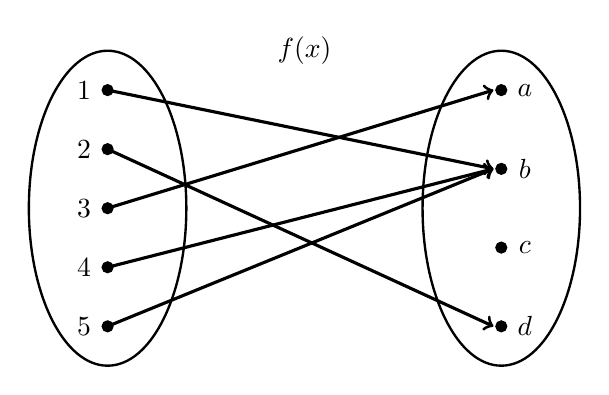
\begin{tikzpicture}
	\node at (2.5,2) {$f(x)$};
	
	% Ellipses
	\draw[line width=0.03cm] (0,0) circle (1 and 2);
	\draw[line width=0.03cm] (5,0) circle (1 and 2);
	
	% Nodes
	\draw[fill=black] (0,1.5) circle (0.07);
	\draw[fill=black] (0,0.75) circle (0.07);
	\draw[fill=black] (0,0) circle (0.07);
	\draw[fill=black] (0,-0.75) circle (0.07);
	\draw[fill=black] (0,-1.5) circle (0.07);
	
	\draw[fill=black] (5,1.5) circle (0.07);
	\draw[fill=black] (5,0.50) circle (0.07);
	\draw[fill=black] (5,-0.5) circle (0.07);
	\draw[fill=black] (5,-1.5) circle (0.07);
	
	% Arrow
	\draw[line width=0.04cm,->] (0,1.5) -- (4.9,0.50);
	\draw[line width=0.04cm,->] (0,0.75) -- (4.9,-1.5);
	\draw[line width=0.04cm,->] (0,0) -- (4.9,1.5);
	\draw[line width=0.04cm,->] (0,-1.5) -- (4.9,0.5);
	\draw[line width= 0.04cm,->,black] (0,-0.75) -- (4.9,0.5);
	
	% Labels
	\node at (-0.3,1.5) {$1$};
	\node at (-0.3,0.75) {$2$};
	\node at (-0.3,0) {$3$};
	\node at (-0.3,-0.75) {$4$};
	\node at (-0.3,-1.5) {$5$};
	
	\node at (5.3,1.5) {$a$};
	\node at (5.3,0.5) {$b$};
	\node at (5.3,-0.5) {$c$};
	\node at (5.3,-1.5) {$d$};
	\end{tikzpicture}
	\]

\begin{enumerate}[(a)]
\item Is the relation a function? Explain. 
\item Find the domain of the relation.
\item Find the codomain of the relation.
\item Find the range of the relation. 
\end{enumerate}



% Question 2
\newpage
\question[10] Consider the relation plotted below.
	\[
	\fbox{
	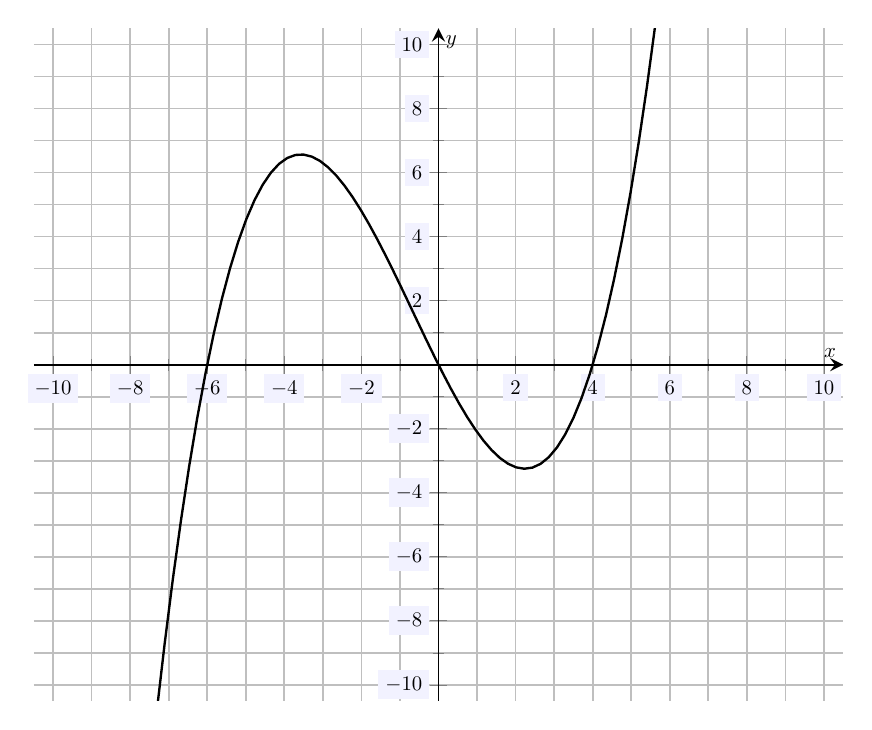
\begin{tikzpicture}[scale=1.5,every node/.style={scale=0.5}]
	\begin{axis}[
	grid=both,
	axis lines=middle,
	ticklabel style={fill=blue!5!white},
	xmin= -10.5, xmax=10.5,
	ymin= -10.5, ymax=10.5,
	xtick={-10,-8,-6,-4,-2,0,2,4,6,8,10},
	ytick={-10,-8,-6,-4,-2,0,2,4,6,8,10},
	minor tick = {-10,-9,...,10},
	xlabel=\(x\),ylabel=\(y\),
	]
	\addplot[line width= 0.02cm,samples=100,domain= -10.5:10.5] ({x},{1/10*x*(x + 6)*(x-4)});
	\end{axis}
	\end{tikzpicture}
	}
	\] 

\begin{enumerate}[(a)]
\item Is this relation a function of $x$? Explain.
\item Is this relation a function of $y$? Explain. 
\item If one were to consider this relation as a function of $x$, would the relation have an inverse? Explain. 
\end{enumerate}



% Question 3
\newpage
\question[10] Let $f(x)$ be the relation given by $f(x)= x(x - 1)(x + 3)$. 
	\begin{enumerate}[(a)]
	\item Is $f(x)$ a function? Explain. 
	\item Find $f(2)$.
	\item Find the $y$-intercept(s) of $f(x)$. 
	\item Find the $x$-intercept(s) of $f(x)$.
	\end{enumerate}



% Question 4
\newpage
\question[10] Let $f(x)$ and $g(x)$ be functions for which a table of values is given below. \par
	\begin{table}[ht]
	\centering
	\begin{tabular}{|c||c|c|c|c|c|c|} \hline 
	$x$ & $-5$ & $-2$ & $0$ & $1$ & $2$ & $3$ \\ \hline \hline
	$f(x)$ & $\phantom{-}6$ & $-1$ & $\phantom{-}3$ & $4$ & $3$ & $-1$ \\ \hline
	$g(x)$ & $-5$ & $\phantom{-}7$ & $-2$ & $4$ & $0$ & $\phantom{-}6$ \\ \hline 
	\end{tabular}
	\end{table} \par
Based on the table above, compute the following:
	\begin{enumerate}[(a)]
	\item $f(-2) - g(3)$
	\item $(f + g)(2)$
	\item $(fg)(-5)$
	\item $(g \circ f)(0)$
	\item $(f \circ g)(0)$
	\end{enumerate}



% Question 5
\newpage
\question[10] Let $g(x)= x^2 + 2x - 3$. 
	\begin{enumerate}[(a)]
	\item Find $g(2)$ and $g(-4)$.
	\item Based on your answer to (a), can $g^{-1}(x)$ exist? Explain. 
	\end{enumerate}



% Question 6
\newpage
\question[10] Consider the function $\ell(x)= \dfrac{4 - 3x}{5}$. 
	\begin{enumerate}[(a)]
	\item Explain why $\ell(x)$ is linear. 
	\item Find the slope of this function.
	\item Find the $y$-intercept of this function.
	\item Find the $x$-intercept of this function.
	\item Does the graph of this function contain the point $(3, -1)$? Explain. 
	\end{enumerate}



% Question 7
\newpage
\question[10] Explain why the function $f(x)= 3(5 - 2x)$ has an inverse. Furthermore, find the inverse. Be sure to show all your work. [You do not need to verify that your inverse is indeed the inverse.]



% Question 8
\newpage
\question[10] Find the exact equation of the line with $x$-intercept $-6$ and $y$-intercept $4$. Show all your work.



% Question 9
\newpage
\question[10] Find the exact equation of the line parallel to the line $4x - 3y= 6$ whose graph contains the point $(-9, -8)$. Show all your work.



% Question 10
\newpage
\question[10] Find the equation of the line perpendicular to $y= \dfrac{5 - 3x}{6}$ whose graph passes through the $x$-intercept of the line $-3x + 9y= 15$. Show all your work.


\end{questions}
\end{document}